%************************************************
\chapter{The main theorem}
%************************************************

Let us quickly recall the main theorem we want to prove.

\begin{theorem*}
    A finitely generated right-angled Coxeter group \(W\) has a finite index subgroup \(W'\) such that \(W'\) is residually finite and rationally solvable (RFRS).
\end{theorem*}

% For the following, we consider the Tits cone \(WC\) corresponding to \(W\), living in \(\R^n\) for \(n = \abs{I}\).
% Before continuing, we want to shortly mention that the fundamental chamber \(C\) has a natural orbifold structure as the quotient \(\faktor{WC}{W}\). % \(WC/W\).
% This will be covered later on in slightly greater detail.
% % By the discussion of last chapter, we know that by taking the quotient \(WC/W\), we are left with the fundamental chamber \(C\).
% In the first section, our goal is to produce a manifold cover \(C' \to C\) of the fundamental chamber.
% This cover will be induced by a finite index subgroup in the right-angled Coxeter group \(W\).


% % ***********************************************
% \subsection{How to be RFRS}
% % ***********************************************

% In this subsection, we want to explain, what it means to be residually finite and rationally solvable for a group.

% \begin{definition}
%     Let \(G\) be a group.
%     Then \(G\) is RFRS, if there exists a sequence \(G = G_0 > G_1 > \ldots\) of subgroups, such that each \(G_i\) is a normal subgroup of \(G\) with finite index, the intersection of all \(G_i\) is trivial and \((G_i)_r^{(1)} := \ker\{G \to \Q \otimes_\Z G_{\text{ab}}\}\) is a subgroup of \(G_{i+1}\).
% \end{definition}

% Thus, we want to show that a right-angled Coxeter group \(W\) has a finite index subgroup, which has such a sequence of subgroups.
% Once we have found a candidate finite index subgroup, to prove the existence of such a sequence, we will construct a sequence of two-fold (orbifold) covers of the fundamental chamber \(C\) of \(W\).
% We will then see that this sequence of covering spaces is cofinal, meaning that it will at some point cover the whole Tits cone, which is the universal cover of the fundamental chamber.

% At this point we will already have much of the desired properties from the RFRS definition.
% By the correspondence of coverings and subgroups of the fundamental group of a space, we see that the cofinal sequence of two-fold covers gives rise to a sequence of subgroups, each of whose has finite index in \(W'\).
% Since the sequence of covering spaces is cofinal, the sequence of subgroups is cofinal as the fundamental group of the Tits cone is trivial.



% ***********************************************
\section{Construction of the manifold cover}
% ***********************************************

Consider the abelianization \(W_{\text{ab}}\) of \(W\), which is isomorphic to \((\Z/2\Z)^{n}\).
Now, the abelianization yields a homomorphism \(\alpha : W \to W_{\text{ab}}\) to whose kernel \(\ker\alpha\), we will turn our attention to in the following.
Note that by the first homomorphism theorem, \(\ker\alpha\) has finite index in \(W\), since
\[\abs{\faktor{W}{\ker\alpha}} = \abs{\faktor{\Z}{2\Z}}^{n} = 2^{n} < \infty.\]
Here we used the fact that \(W\) is finitely generated, whence \(n = \abs{I} = \abs{S} < \infty\).

Furthermore, note that for each \(J \subset I\) with \(W_J\) finite, we have an isomorphism between \(W_J\) and \((\faktor{\Z}{2\Z})^{\abs{J}}\).
Thus, the restriction of \(\alpha\) to each such subgroup \(\alpha\vert_{W_J}\) is an injective homomorphism.
We now use that in the right-angled case, the isotropy subgroups of codimension-\(k\) faces are all of this form.
This can be seen, as the isotropy subgroup of a codimension-\(k\) face \(F\) is generated by the reflections in the \(k\) codimension-\(1\) faces, whose intersection forms \(F\).
As all these codimension-\(1\) faces meet at angle \(\frac{\pi}{2}\), the generators commute pairwise.
Therefore, all isotropy subgroups inject into the abelianization of \(W\).
This implies that the intersection of an isotropy subgroup with the kernel of \(\alpha\) is trivial and consequently no isotropy group is contained in the kernel \(\ker\alpha\).
Since finite subgroups are contained in isotropy subgroups, the kernel \(\ker\alpha\) acts freely on the Tits cone \(WC\) corresponding to \(W\).

In particular, by \Cref{thm:stabilizer} the action of \(W\) on the interior of its Tits cone \(int(WC)\) is properly discontinuously.
By \Cref{thm:convexity} the Tits cone is also a convex cone, implying that it has trivial fundamental group, whence is simply-connected.
Having all this information, we are able to apply \Cref{lem:covering} to obtain the covering
\[int(WC) \;\longrightarrow\; \faktor{int(WC)}{\ker\alpha} \qquad x \mapsto \text{Orb}_{\ker\alpha}(x).\]
% Using the local homeomorphism property of a covering map and the fact that the Tits cone \(WC\) is a subspace of \(\R^n\), we conclude that the quotient \(\faktor{int(WC)}{\ker\alpha}\) is indeed a manifold.
We conclude the result of this section in the following proposition.

\begin{proposition}
    Let \(W\) be a right-angled Coxeter group with corresponding Tits cone \(WC\). % and fundamental chamber \(C\).
    Then, there is a finite index subgroup \(W' \leq W\), acting by covering action on the interior of the Tits cone, implying that the quotient \(\faktor{int(WC)}{W'}\;\) is a manifold.
    In particular, \(W' = \ker\{W \to W_{\text{ab}}\} = \ker\alpha\).
    % In particular, we can take \(W'\) to be the kernel of the abelianization homomorphism \(\alpha : W \to W_{\text{ab}}\).
\end{proposition}


% ***********************************************
\section{Some orbifold theory}
% ***********************************************

In this section, we want to elaborate more on the natural orbifold structure of the fundamental chamber \(C\).
We start by giving a formal definition of an orbifold.
We break the definition down into smaller pieces, starting with local models, sometimes called (orbifold) charts.

\begin{definition}
    A \emph{local model} is a pair \((\widetilde{U}, \Gamma)\), where \(\widetilde{U} \subset \R^n\) is open and \(\Gamma\) is a finite subgroup of the group of diffeomorphisms of \(\widetilde{U}\), denoted \emph{diffeo}\((\widetilde{U})\), acting on \(\widetilde{U}\).
    By abusing notation, we will sometimes say that the quotient \(U = \faktor{\widetilde{U}}{\Gamma}\;\) is the local model.
\end{definition}

Now that we have defined the local structure of an orbifold, we want to translate between these local models.
This is being made precise by orbifold maps.

\begin{definition}
    An \emph{orbifold map} between local models \((\widetilde{U}_i, \Gamma_i), (\widetilde{U}_j, \Gamma_j)\) is a pair of maps \((\widetilde{\psi}, \varphi)\),
    consisting of a smooth map \(\widetilde{\psi} : \widetilde{U}_i \to \widetilde{U}_j\) and a homomorphism of groups \(\varphi : \Gamma_i \to \Gamma_j\).
    We enforce the map \(\widetilde{\psi}\) to be \(\varphi\)-equivariant, meaning that for all \(g \in \Gamma_i\) and all \(\widetilde{x} \in \widetilde{U}_i\), \(\widetilde{\psi}(g\widetilde{x}) = \varphi(g)\widetilde{\psi}(\widetilde{x})\) holds.
    Then \(\widetilde{\psi}\) induces a map \(\psi : \faktor{\widetilde{U}_i}{\Gamma_i} \to \faktor{\widetilde{U}_j}{\Gamma_j}\), between the local models.
    When all three of these maps are injective, we call \(\psi\) a local isomorphism.
\end{definition}

Now that we have these local definitions, we `glue' them together, to obtain an orbifold.
Before we do so, we recall some notions from topology.

Suppose, we are given an open cover \(\{U_i\}\) of a topological space \(X\).
It is said to be \emph{locally finite}, if every \(x \in X\) admits a neighborhood \(N\) such that \(N \cap U_i\) is empty for all but finitely many \(i\).
The open cover \(\{U_i\}\) is a \emph{refinement} of an open cover \(\{V_j\}\) of \(X\), if for every \(V_j\) there is a \(U_i\) with \(U_i \subseteq V_j\).
Now, the topological space \(X\) is said to be \emph{paracompact}, if every open cover of \(X\) admits such a locally finite refinement.

\begin{definition}
    An \(n\)-dimensional \emph{(smooth) orbifold} \(Q\) is a pair \((X_Q, \mathcal{A})\).
    The space \(X_Q\) is a paracompact Hausdorff space, called the \emph{underlying space}.
    The set \(\mathcal{A}\) is called an \emph{orbifold atlas}, consisting of charts \((U_i, \phi_i)\), indexed by some set \(I\) and satisfying the following conditions:
    \begin{itemize}
        \item the \(U_i\) form an open cover of the underlying space \(X_Q\),\vspace*{-.7em}
        \item for each \(U_i\) there exists a local model \(\faktor{\widetilde{U}_i}{\Gamma_i}\) with a homeomorphism \(\phi_i : U_i \to \faktor{\widetilde{U}_i}{\Gamma_i}\) and
        \item charts have to be compatible, meaning that for \(U_i \subset U_j\) the inclusion is a local isomorphism.
    \end{itemize}
\end{definition}

To sketch the connection between manifolds and orbifolds, let us mention one more thing.

\begin{definition}
    The \emph{local group} \(loc(x)\) of some \(x\) in a local model \(\faktor{\widetilde{U}}{\Gamma}\;\) is the isotropy group of any \(\widetilde{x}\) in \(\widetilde{U}\), getting projected onto \(x\).
    The \emph{singular locus} \(\Sigma (Q)\) of an orbifold \(Q\) consists of all points in the underlying space \(X_Q\) with non-trivial local group, i.e. \(\Sigma(Q) = \{x \in X_Q \;\vert\; loc(x) \neq \{1\}\}\).
\end{definition}

By this definition, we see that an orbifold with empty singular locus is just a manifold.
Furthermore, when thinking about an orbifold, we can just think about the underlying space and label each element in the singular locus by its local group.

Many basic examples arise by taking the quotient relative to a properly discontinuous group action on \(\R^n\).
We want to mention at least some examples.

\begin{example} % TODO: add pictures
    \begin{enumerate}
        \item Consider the flat plane \(\R^2\) with the action of a cyclic group \(\faktor{\Z}{n\Z}\) by rotation about the origin.
            The arising orbifold is a cone with singular point the origin and cone angle \(\frac{2\pi}{n}\).
        
        \item Consider the sphere \(S^2\) with the action of a cyclic group \(\faktor{\Z}{2\Z}\) by rotation about the north pole \(N\).
            The arising orbifold now is called a \emph{teardrop} with singular point, the north pole \(N\).
            
        % \item Cosider the torus \(\mathbb{T}^2 \cong \faktor{\R^2}{\Z^2}\) with the action of the group \(\faktor{\Z}{2\Z}\) acting by reflection in the midpoints of the y-axis of \(\Z^2\)-lattice in \(\R^2\).
    \end{enumerate}
\end{example}

By starting with a topological space \(X\), this is actually a more general way to construct orbifolds.
Given a properly discontinuously action of a group \(G\) on \(X\), simply pass to the quotient space \(\faktor{X}{G}\) to obtain an orbifold.
In contrast, to obtain a manifold, one has to demand the action to be free as well.
This is not the only analogy between manifolds and orbifolds.
The concept of orbifold coverings translates almost one to one from the ordinary case.

\begin{definition}
    An orbifold covering \(p: Q' \to Q\) is a continuous map on the underlying spaces \(X_{Q'} \to X_Q\), such that for each point \(x \in X_Q\) there is a local model \(U = \faktor{\widetilde{U}}{\Gamma}\) around \(x\) and each component \(V_i\) of \(p^{-1}(U)\) is homeomorphic to \(\faktor{\widetilde{U}}{\Gamma_i}\) for a subgroup \(\Gamma_i\) of \(\Gamma\).
    Furthermore, the restriction \(p\vert_{V_i} : V_i \to U\) corresponds to the natural projection \(\faktor{\widetilde{U}}{\Gamma_i} \to \faktor{\widetilde{U}}{\Gamma}\).
\end{definition}

\begin{remark}\label{rmk:covers}
    We want to mention here, that the universal cover of an orbifold is exactly what we think of, i.e. the initial object in the category of orbifold coverings.
    Moreover, there is a notion of orbifold fundamental groups as well and they behave to orbifold covers the same as fundamental groups to coverings in the ordinary case.
    In particular, subgroups (of index \(n\)) of the orbifold fundamental group correspond to (\(n\)-sheeted) orbifold coverings.
\end{remark}
    
Having all this in mind, we have two ways of approaching the fundamental chamber \(C\).
One way, it obtains its natural orbifold structure as the quotient \(\faktor{int(WC)}{W}\), where we observe that the orbifold fundamental group of \(C\) is precisely \(W\).
As the Tits cone is simply connected, it is the universal cover of \(C\).
On the other hand, the fundamental chamber is the quotient of the manifold \(\faktor{int(WC)}{\ker\alpha}\) by a finite group action.
\vspace*{\parskip}

\begin{figure}[h!]
    \begin{minipage}[c]{.58\textwidth}
        Since \(\ker\alpha\) is a finite index subgroup of \(W\), \Cref{rmk:covers} implies that we get a covering map \(p\) so that the diagram on the right commutes.
        Thus, both of the approaches to the fundamental chamber \(C\) agree in the sense that the projection map \(int(WC) \to \faktor{int(WC)}{W}\) factors through the manifold cover, constructed earlier.
    \end{minipage}\quad
    \begin{minipage}{.4\textwidth}\vspace*{-1em}
        \begin{tikzcd}
            int(WC) \arrow[r] \arrow[d] & \faktor{int(WC)}{W} \\
            \faktor{int(WC)}{\ker\alpha} \arrow[ru, "p"', dashed]
        \end{tikzcd}
    \end{minipage}
\end{figure}


% ***********************************************
\section{The cofinal cover}
% ***********************************************

In this section, we want to at least \emph{sketch} the proof of the existence of a cofinal sequence of two-fold covers, arising by iteratively reflecting in faces.
Some more results from the theory of orbifolds are needed for the whole proof.
We will state and use them without proof.

In the following, doubling along a face means the construction of a sequence of polytopes \(P_k = P_{k-1} \cup g_{k-1}(P_{k-1})\), where \(g_{k-1}\) is the reflection in one of the faces of the previous polytope \(P_{k-1}\).
The following proposition will tell us, that in the case of a right-angled Coxeter group, we are able to double the fundamental chamber \(C\) in one of its faces and are still able to cover the whole Tits cone \(WC\) by reflecting in the faces of the resulting chamber.

\begin{proposition}\label{prop:double}
    Let \(P_k \subset \R^n\) be a polytope with orbifold structure, orbifold fundamental group \(\pi_1^{\text{orb}}(P_k)\) and universal cover \(\widetilde{P}\).
    Then, the fundamental group \(\pi_1^{\text{orb}}(P_{k+1})\) is isomorphic to the group generated by reflections in the faces of the double \(P_{k+1}\).
    Furthermore, the fundamental group \(\pi_1^{\text{orb}}(P_{k+1})\) of the double is an index-\(2\) subgroup of \(\pi_1^{\text{orb}}(P_k)\) and the following two conditions are satisfied.
    \begin{enumerate}
        \item \(\forall k \in \N: \forall g \in \pi_1^{\text{orb}}(P_k): g(\mathring{P_k}) \cap \mathring{P_k} \neq \emptyset \implies g = 1\), and
        \item \(\forall k \in \N: \bigcup_{g \in \pi_1^{\text{orb}}(P_k)} g(P_{k}) = \widetilde{P}\).
    \end{enumerate}
\end{proposition}
\begin{proof}
    We won't proof this here.
\end{proof}

To state the other helping lemma we will need, we first want to show that each chamber in the Tits cone can uniquely be labeled by elements of its corresponding group.

\begin{lemma}\label{lem:labels}
    Let \(W\) be a Coxeter group and \(WC\) its Tits cone.
    The chambers of the form \(w(C)\) in the Tits cone can be labeled uniquely by elements in \(W\).
\end{lemma}
\begin{proof}
    Let \(v(C), w(C)\) be chambers in \(WC\) for \(v, w \in W\), such that \(v \neq w\) and \(w(C) = v(C)\).\newline
    But then, by \Cref{thm:stabilizer} we have that
    \[w(\mathring{C}) \cap v(\mathring{C}) = w(\mathring{C} \cap w^{-1}v(\mathring{C})) \neq \emptyset \implies w^{-1}v = 1 \iff w = v.\]
    Thus, the chambers can be labeled in a unique way.
\end{proof}

We proceed with another helpful result, whose proof relies on the aforementioned results.

\begin{lemma}
    Let \(C \subset \R^n\) be the fundamental chamber of a Coxeter group \(W\).
    The non-trivial labels \(w_i \neq 1_W\) of the chambers, defining the polytope \(P = \bigcup_{i=1}^n w_i(C)\), are \emph{not} contained in the reflection group, generated by reflecting in its faces.
\end{lemma}
\begin{proof}
    Note that by \Cref{lem:labels}, the chambers of the form \(w(C)\) are uniquely labeled by \(w \in W\).
    Thus, let \(P := \bigcup_{i = 1}^n w_i(C)\) be as in the lemma and \(w_i\) one of its defining labels.
    Assume, \(w_i \neq 1_W\) is contained in the reflection group generated by reflecting in the faces of \(P\).
    But then we have that \(w_i(\mathring{P}) \cap \mathring{P} \neq \emptyset\), contradicting \Cref{prop:double}.
\end{proof}

Using this insight, we define a graph \(G\) with vertices \(V(G) := \{w(C) \;\vert\; w \in W\}\) and edges \(E(G) := W \times S\).
The endpoint map is given by \(\delta : W \times S \to 2^{V(G)},\; (w, s) \mapsto (w(C), ws(C))\).
Thus, two vertices \(w(C)\) and \(v(C)\) have an edge, if there is an \(s \in S\), such that \(ws = v\).
Then, clearly we have \(wsw^{-1}w(C) = ws(C) = v(C)\).
Note that the element \(wsw^{-1}\) is the only element, that flips the edge \(\{w(C), ws(C)\}\).
Thus, the map \(W \times S \to W, \; (w, s) \mapsto wsw^{-1}\) defines a labeling of the edges by elements in \(W\).
We will call the combinatorial graph of \(G\) (meaning that every double edge gets collapsed) the \emph{chamber graph} Cham\((W, S)\) of \(W\).

It is obvious, that this graph is isomorphic to the combinatorial Cayley graph of the group \(W\) and we see that the Cayley graph `embeds' into the Tits cone \(WC\).
This will be useful to prove the next theorem.

\begin{theorem}\label{thm:cofinal}
    By doubling in a face of the fundamental chamber and iteratively doubling the resulting chamber, we will at some point cover every chamber in the Tits cone \(WC\).
\end{theorem}
\begin{proof}
    The proof is by induction on the word length \(\ell(w)\).
    For \(\ell(w) = 0\), the corresponding chamber is the fundamental chamber \(C\), which is covered by itself.
    \IH{Chambers with labels \(v\) of length \(\ell(v) = k - 1\) are covered by a polytope \(P = \bigcup_{i=1}^n w_i(C)\).}\par\noindent
    We need to show that chambers of the form \(w(C)\) with \(\ell(w) = k\) can be covered by reflecting in a face of the polytope \(P\).
    Using the chamber graph Cham\((W, S)\), constructed above, we deduce that for each such \(w\), there is a \(v \in W\) of length \(\ell(v) = k - 1\), connected to \(w\) by an edge in Cham\((W, S)\). % , labeled by \(ws_iw^{-1}\) for an \(i \in I\).
    This is due to the fact that the chamber graph is isomorphic to the Cayley graph of  \(W\) and the length function of \(W\) is induced by the Cayley graph.
    But then, the chamber \(w(C)\) is adjacent to the chamber \(v(C)\) and the latter is contained in \(P\) by \textbf{(IH)}.
    Thus, either \(w(C)\) itself is already contained in \(P\) or we reflect in the face shared by \(w(C)\) and \(v(C)\) to cover \(w(C)\) with the double \(P'\) of \(P\).
    Now, continuing with the next element \(w\) of length \(k\), we eventually double \(P'\) and repeat this for all such \(w\).
    This iterative doubling process is valid by \Cref{prop:double} and by induction every chamber \(g(C)\) for \(g \in W\) can be covered.
\end{proof}

Thus, we conclude that the doubling sequence starting in the fundamental chamber \(C\) is a cofinal sequence of two-fold covers.

\begin{remark}\label{rmk:groupseries}
    Using \Cref{prop:double}, we see that the cofinality of this sequence translates to the group side.
    More precisely, this sequence of two-fold covers induces a sequence of index-\(2\) subgroups via the fundamental groups of the covering spaces.
    As we will at some point cover the whole Tits cone, whose fundamental group is trivial, the intersection of all these groups is trivial.
    Furthermore, as index-\(2\) subgroups are normal, at this point we have constructed a descending normal series of groups.
\end{remark}

\begin{figure}[ht!]
    \centering
    \subfloat[The fundamnetal chamber \(C\).]{{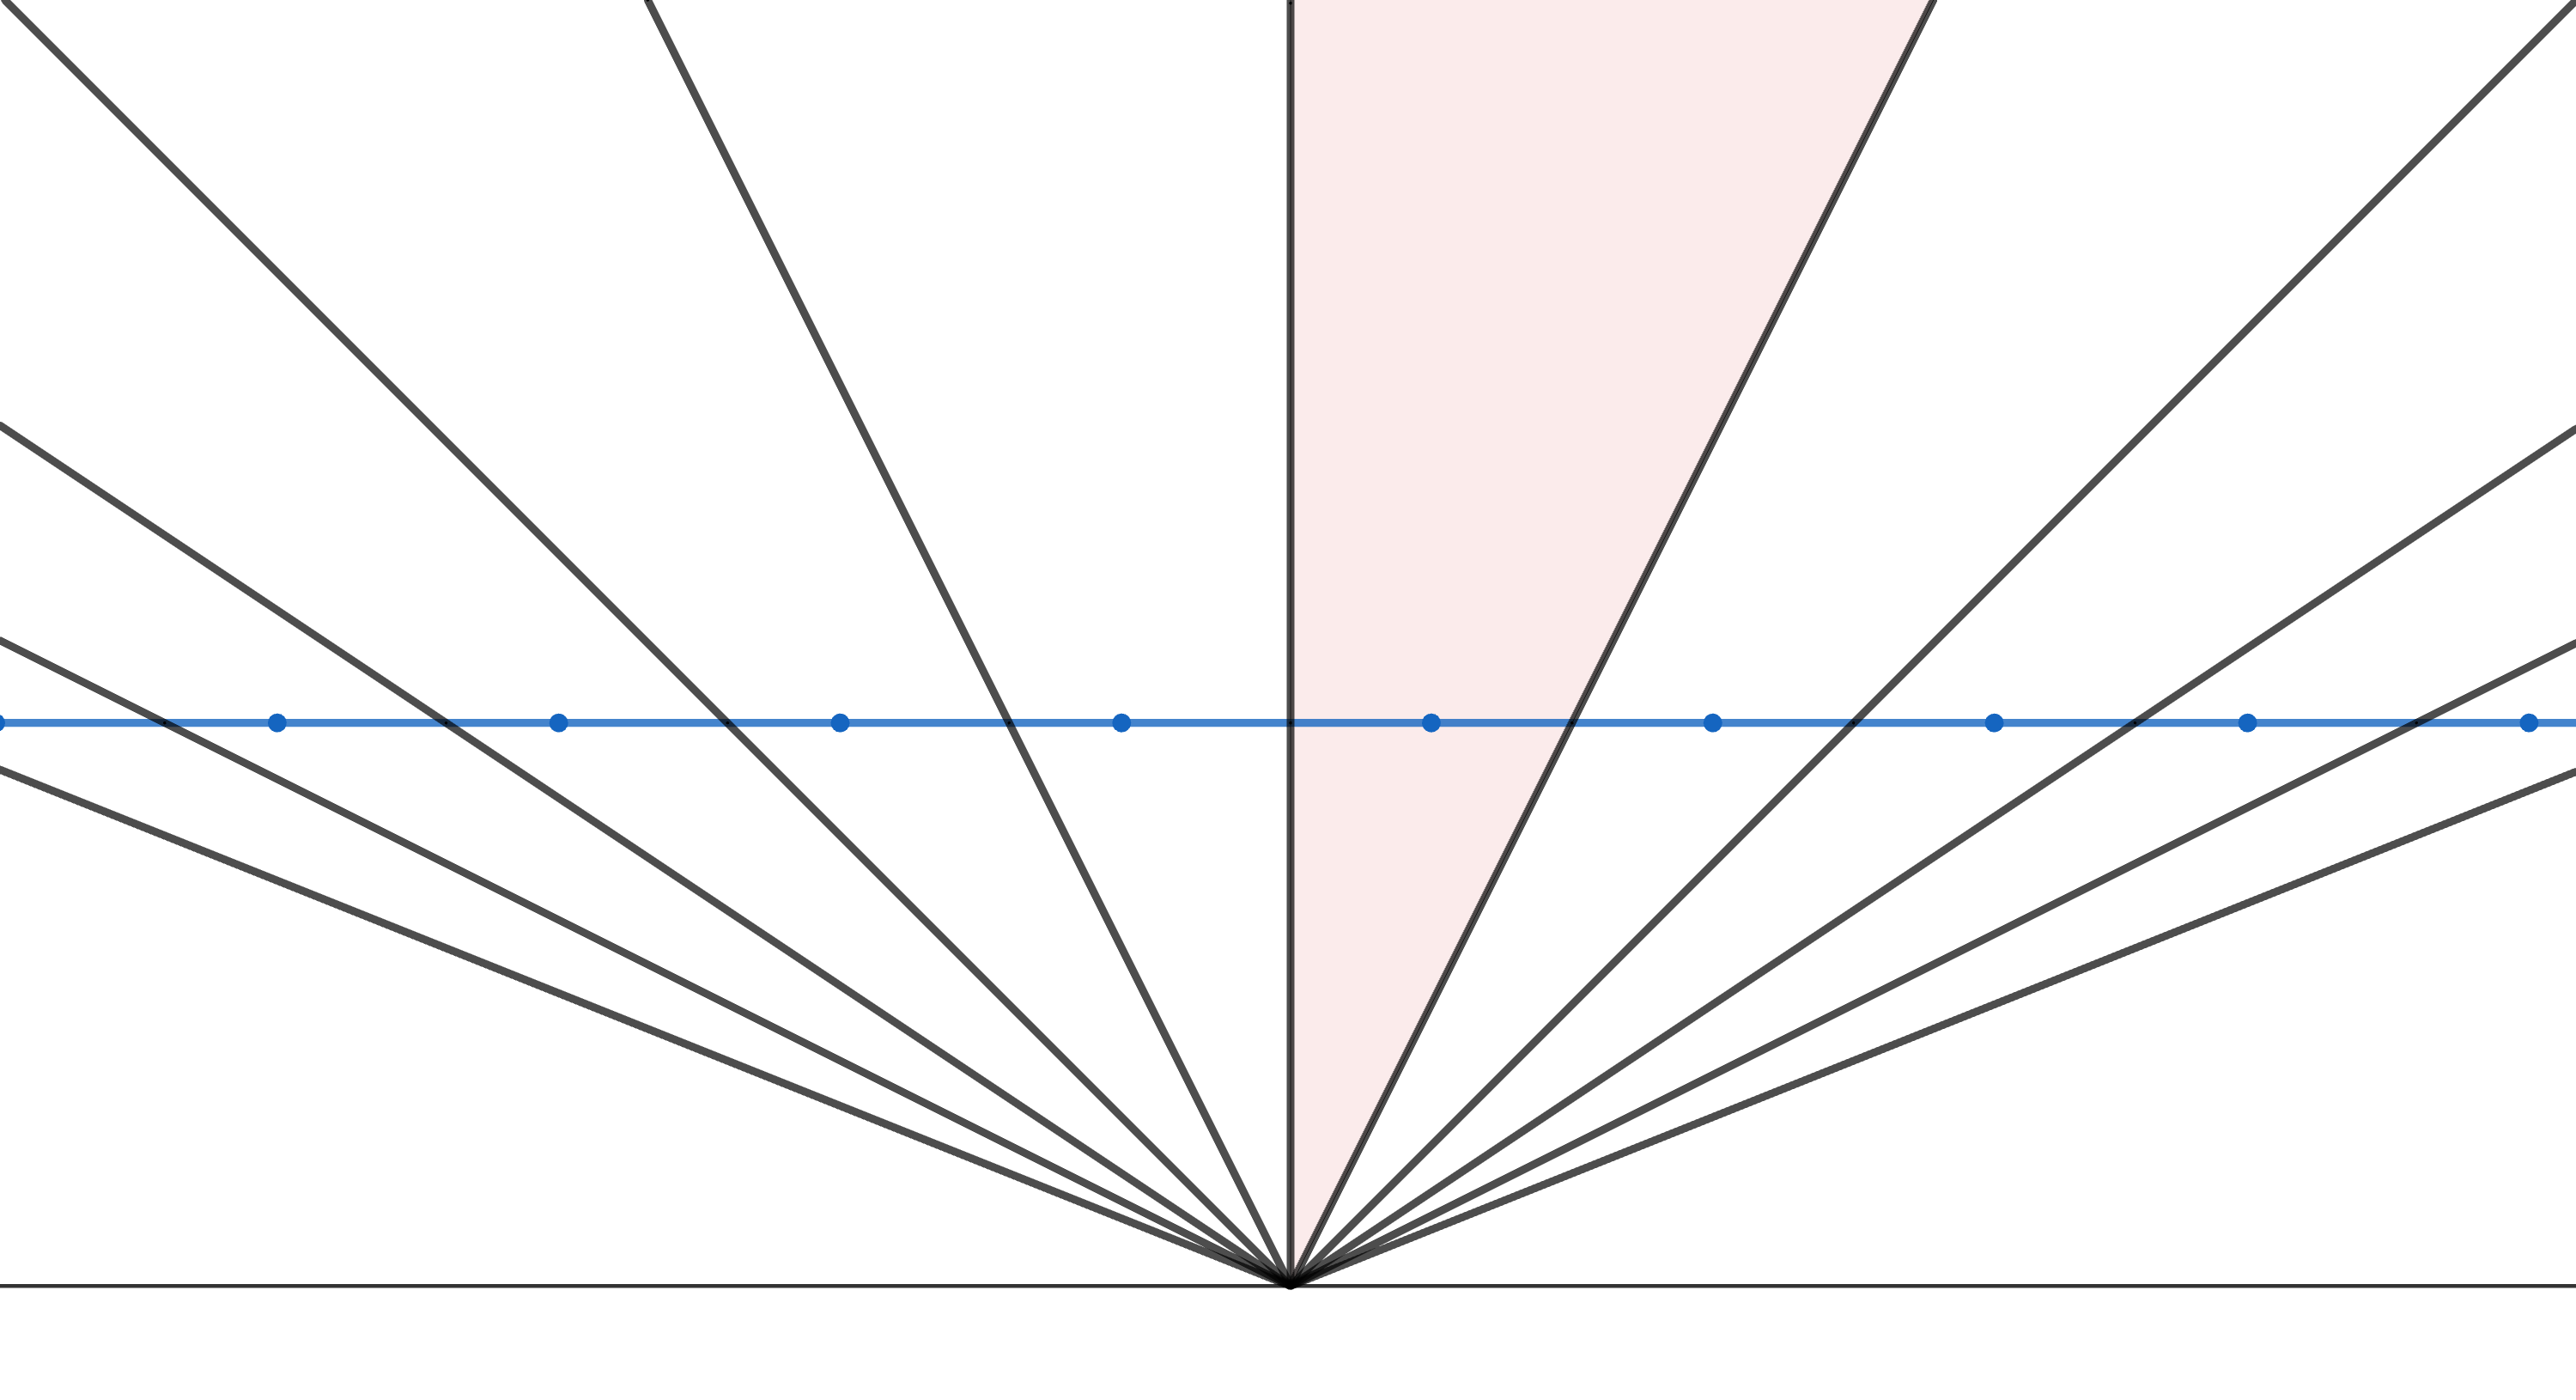
\includegraphics[width=6cm]{gfx/chamber graph - 1.png}}}\qquad
    \subfloat[The double polytope \(P = C \cup s_1(C)\)]{{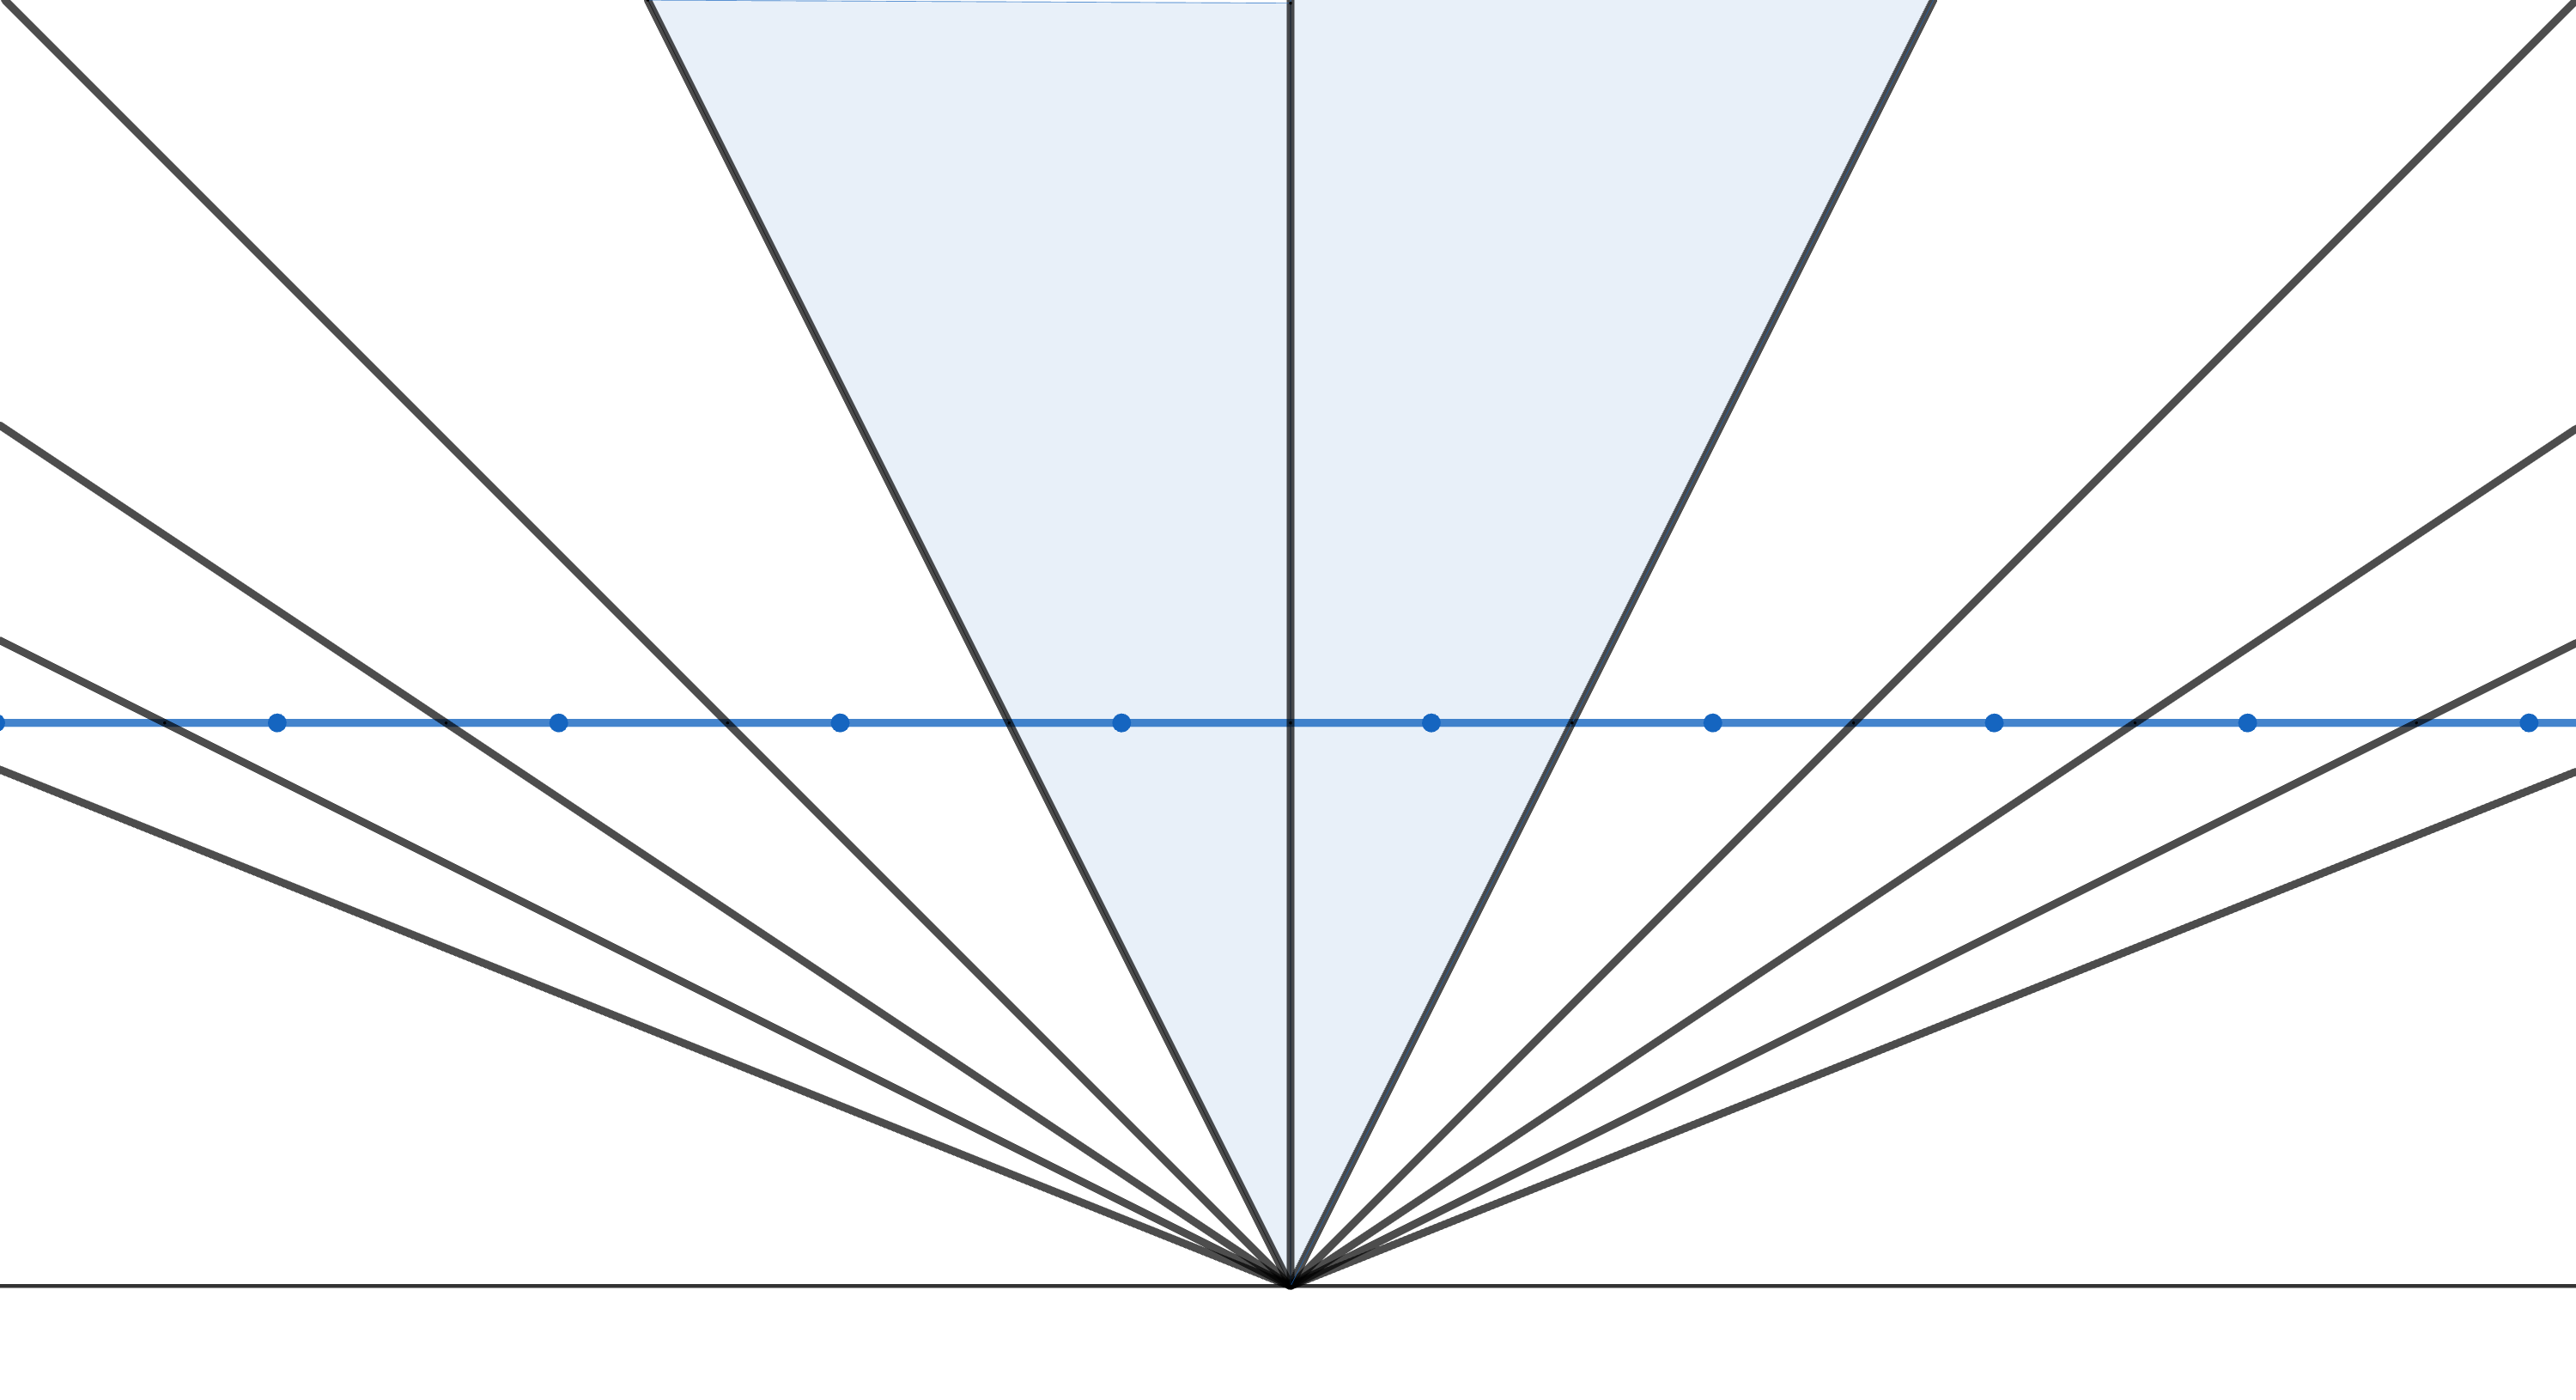
\includegraphics[width=6cm]{gfx/chamber graph - 2.png}}}\newline
    \subfloat[The double polytope \(P' = P \cup s_1s_2s_1(P)\)]{{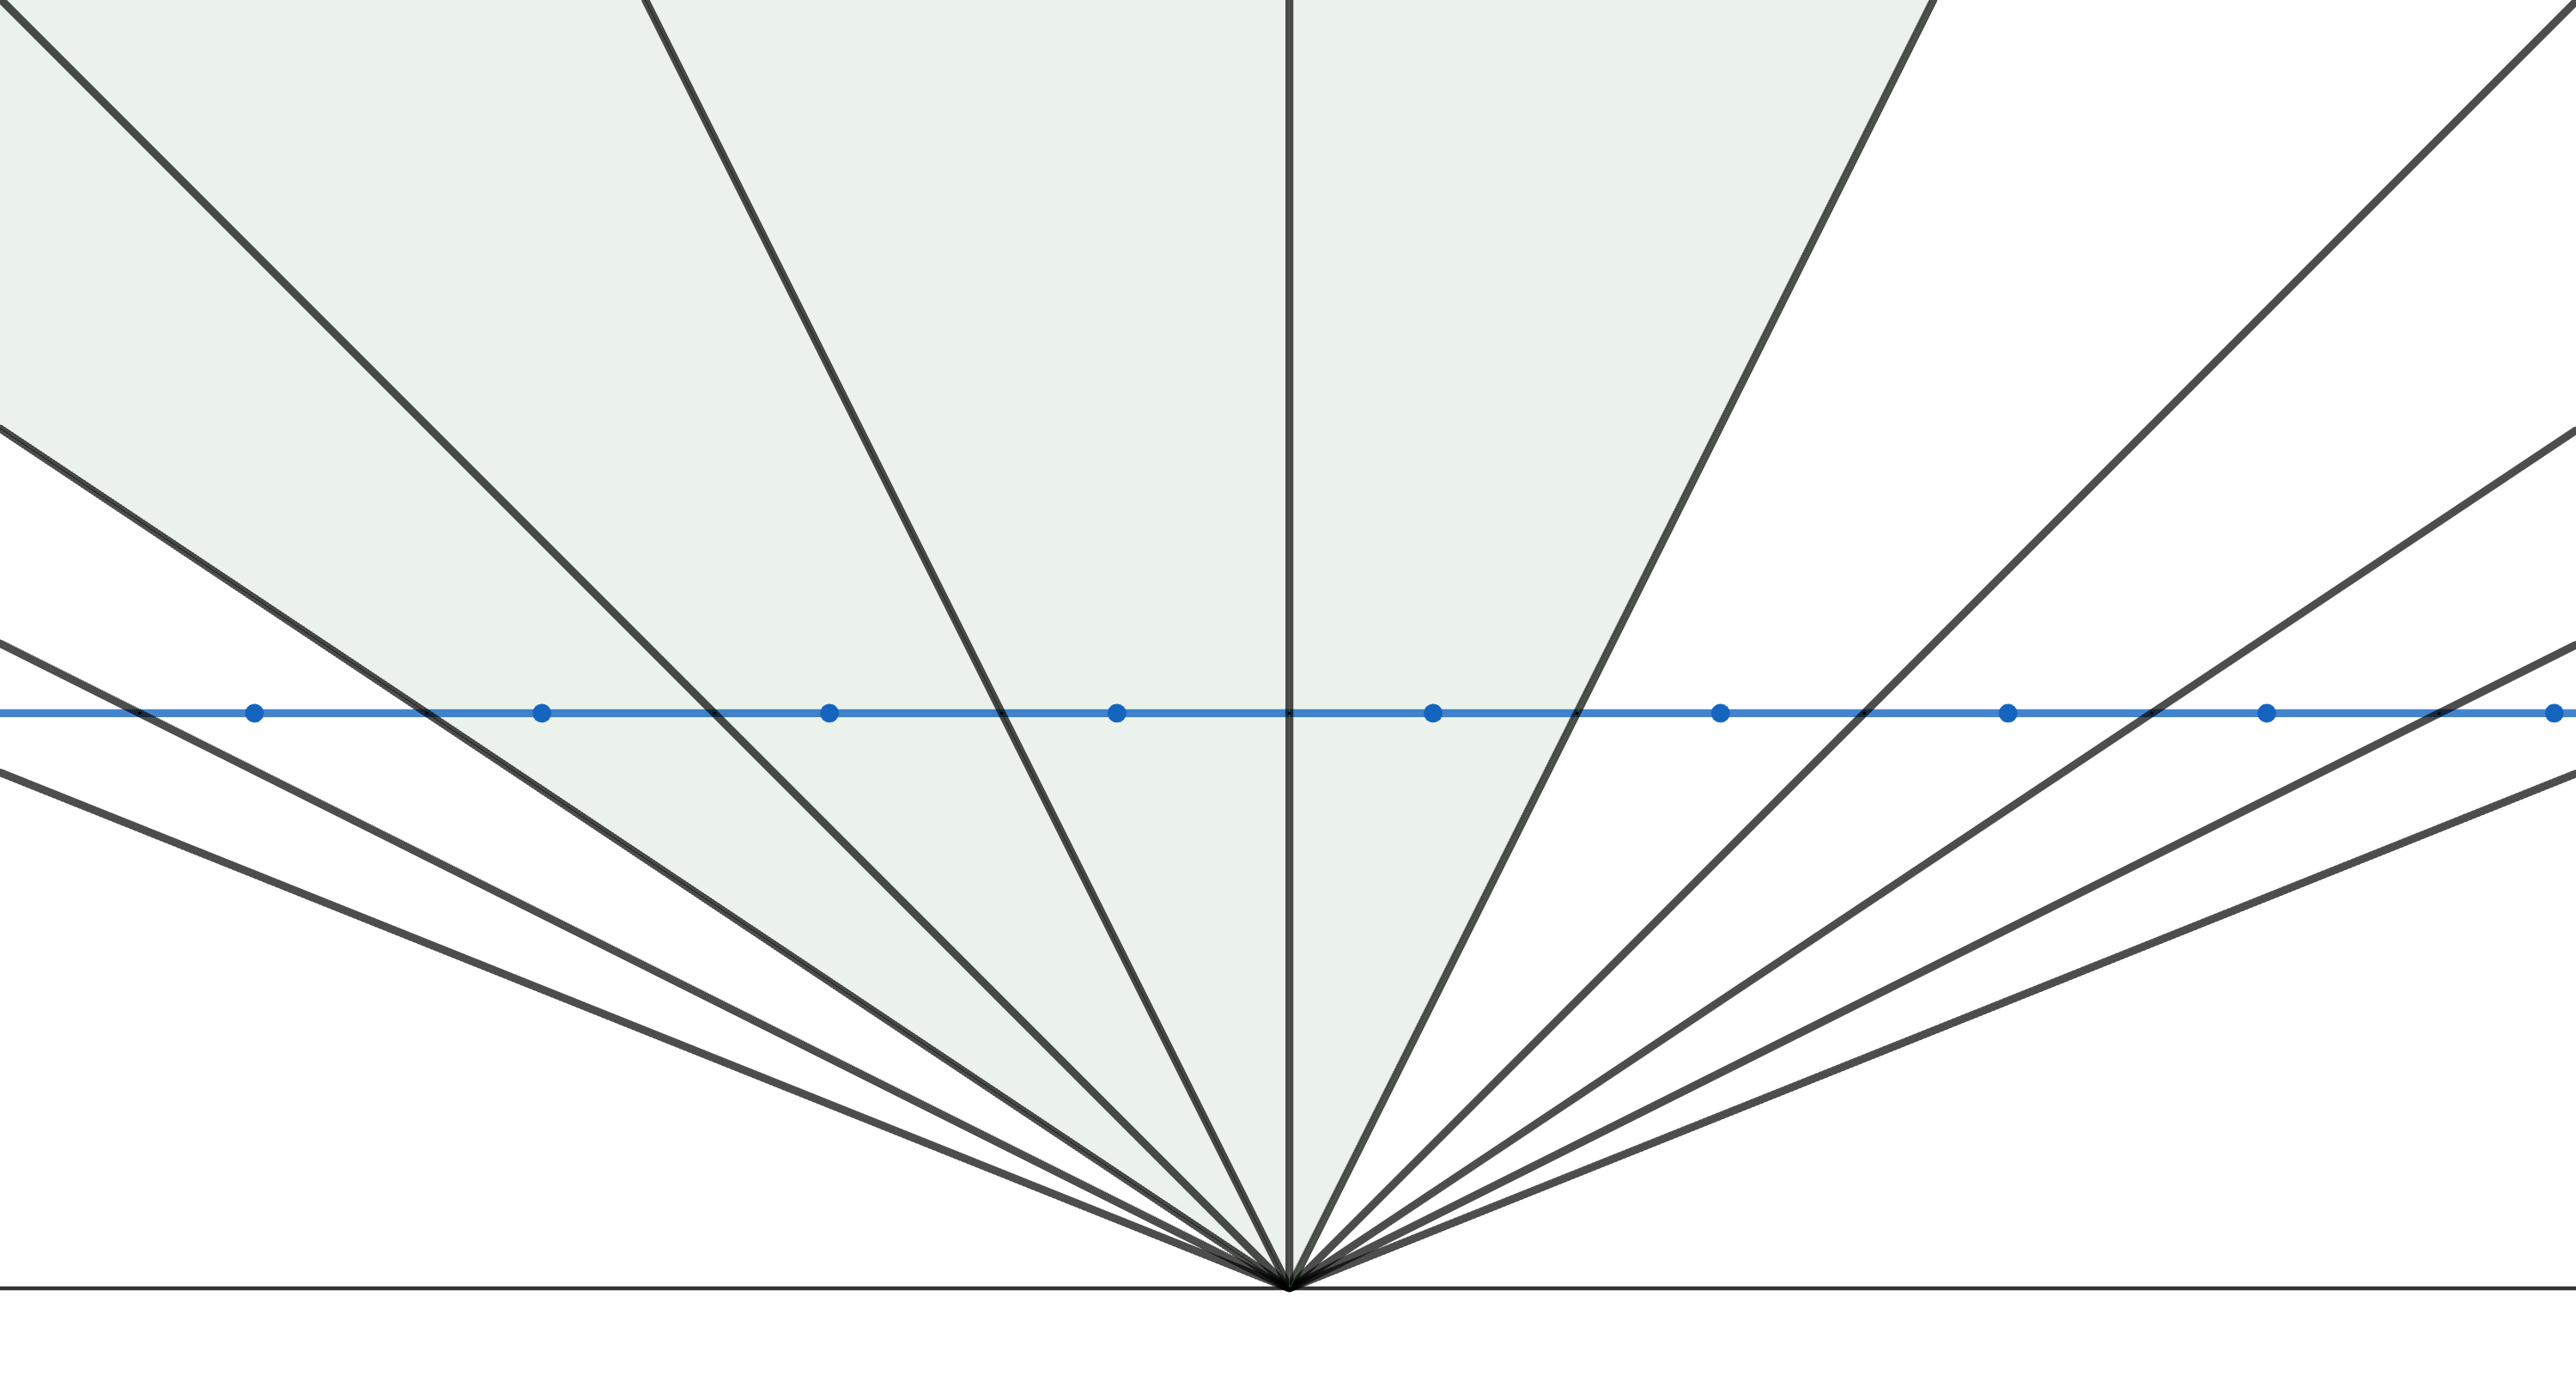
\includegraphics[width=6cm]{gfx/chamber graph - 3.png}}}
    \caption{An example doubling sequence in \(D_\infty\)}
\end{figure}

\newpage
% ***********************************************
\section{The manifold sequence}
% ***********************************************

% The goal of this section is to construct a descending series of groups \(W = G_0 \geq G_1 \geq G_2 \geq \ldots\), where \(G_i \mathrel{\unlhd} W\), \(\bigcap_{i} G_i = \{1\}\) and \([G : G_i] < \infty\).
% Recall that \(\ker\alpha = \ker\{W \to W_{\text{ab}}\}\) induces a manifold cover of the fundamental chamber \(C\).
% Moreover, \(\ker\alpha\) is a normal subgroup of \(W\), suggesting the following construction.

% Following \Cref{rmk:groupseries}, take the descending normal series of fundamental groups \(\pi_1^{\text{orb}}(P_k)\) induced by the doubling sequence \(P_k\).
% The intersection of \(\ker\alpha\) with \(\pi_1^{\text{orb}}(P_k)\) is a subgroup of \(\ker\alpha\), in particular normal in \(W\).

